
% --------------------------------------------------------------------
% This is a simple Beamer document that uses beamerthemesigma.sty
% Reading the comments should help you create a presentation even if
% you've never used Beamer before.
% --------------------------------------------------------------------
% Set our document class to Beamer
\documentclass[aspectratio=169, handout]{beamer}

% Some packages for nice font encodings in the final PDF
\usepackage[utf8]{inputenc}
\usepackage[T1]{fontenc}

% From Jeff E
\usepackage{algo}

\usepackage{sigmastyle}

% To insert images
\usepackage{graphicx}

% Useful packages from the AMS
\usepackage{amsmath,amssymb,amsthm}

% Package for code highlighting
\usepackage{minted}
\setminted{linenos=true, breaklines=true, breakanywhere=true, style=default}
\usemintedstyle{monokai}

% Set a title
\title{Regular Languages Pt. 1}

% The subtitle is generally where I'd expect you to put the week
% number, thus:
\subtitle{Week 1}
% \texorpdfstring to remove compilation warnings if you have math here

% Whoever worked on the presentation:
\author{Anakin}

% A date, if you'd like.
\date{}

% An institute name, if you're so inclined
% \institute{University of Illinois Urbana-Champaign}

% Use the SIGma theme for this Beamer presentation
\usetheme{sigma}
% --------------------------------------------------------------------
% Begin document
\begin{document}

% Beamer calls each slide a "frame", defined within the environment:
% \begin{frame}
%   <frame content here>
% \end{frame}

% This frame is just the title.
\begin{frame}
\titlepage
\end{frame}

% A frame with the table of contents.
% This frame's title is "Outline".
\begin{frame}{Outline}
  \tableofcontents
\end{frame}

% The frame title is a flag.
\begin{frame}{Updates}
  % Let's put some real content in this frame:
  \begin{itemize}
    \item Why Sipser? \pause
    \item Combinational Algorithms \pause
    \item Discord
  \end{itemize}
  \hfill
  
\includegraphics[scale=0.15]{sigma-code2.png}
\end{frame}

% Start a section: *sections* (subsections, etc.) are what show up in the TOC.
\section{Regex}
% Section pages can be printed thus:
\frame{\sectionpage}
% There's a way to automate this, see:
% https://tex.stackexchange.com/questions/178800/creating-sections-each-with-title-pages-in-beamers-slides/178803

\begin{frame}{\textul{Reg}ular \textul{Ex}pressions}

\begin{center}
    $ \Sigma^* = \texttt{(0 + 1)}^* = $ The set of all finite binary strings
\end{center}
    
    \begin{itemize}
        \item Many of us have probably seen regex appear in programming when we want to do \textbf{string matching} \pause
        \item Turns out that \textbf{languages} (a set of strings) are an extremely powerful idea at the center of CS \pause
        \item Languages recognized by regular expressions are called regular languages \pause
        \item Let's look at a simplified version of regex with only 3 operations
    \end{itemize}
    
\end{frame}

\begin{frame}{}
    Recursively build regex:
    \begin{itemize}
        \item Base Cases: The emptyset: $\emptyset$, the empty string $\varepsilon$, or a string $s$ \pause
        \item Operations:
        \begin{itemize}
            \item \textbf{Concatenation:} We can attach strings in one language $R_1$ to strings in another $R_2$ and form $R_1 R_2$
            \begin{itemize}
                \item Example: $R_1 = \set{\texttt{0, 00}}$, $R_2 = \set{\texttt{1, 11}}$, $R_1 R_2 = \set{\texttt{01, 011, 001, 0011}}$ \pause
            \end{itemize}
            \item \textbf{Union:} We take one language $R_1$ and add all the words of another language another $R2$ and form $R_1 + R_2$
            \begin{itemize}
                \item Example: $R_1 = \set{\texttt{0, 00}}$, $R_2 = \set{\texttt{1, 11}}$, $R_1 + R_2 = \set{\texttt{0, 00, 1, 11}}$ \pause
            \end{itemize}
            \item \textbf{Star:} We take a language $R$ and string words in itself 0 or more times and form $R^*$
            \begin{itemize}
                \item Example: $R = \set{\texttt{0, 1}}$, $R^* = $ every possible finite binary string!
            \end{itemize}
        \end{itemize}
    \end{itemize}
\end{frame}

\begin{frame}{}
      \begin{center}
    {\color{sigma@mainblue} \LARGE Questions?}
  \end{center}
\end{frame}

\begin{frame}{Questions!}
    Try to write out some strings in the following languages and come up with a more intuitive way to understand the language
    
    Example: 
    \begin{align*}
    \texttt{0}^* + \texttt{0}^* 1 \texttt{0}^* &= \set{\varepsilon, \texttt{0, 00, 000, \ldots, 1, 01, 10, 0010, \ldots}} \\
        &= \text{Strings with at most a single }\texttt{1}
    \end{align*}
    
    Note: We use $\Sigma = \texttt{(0 +  1)}$ \pause
    
    \begin{enumerate}
        \item $( \Sigma \Sigma \Sigma)^*$
        \item $\texttt{0 + 1 + 0} \Sigma^* \texttt{0 + 1} \Sigma^* \texttt{1}$
    \end{enumerate}
\end{frame}

\section{Automata}
% Section pages can be printed thus:
\frame{\sectionpage}

\begin{frame}{\textul{D}eterministic \textul{F}inite \textul{A}utomata}

\textbf{Problem:} How can we tell if a string is in some regular language? \pause


\textbf{Solution:} Deterministic Finite Automata (DFA)

\end{frame}

\begin{frame}{}
    We could define this fully formally but these are better introduced an intuitive level \pause
    
    \textbf{GOAL: } Identify binary strings containing an odd number of $\texttt{1}$'s
\end{frame}

\begin{frame}{Odd number of $\texttt{1}$'s}
    \begin{center}
        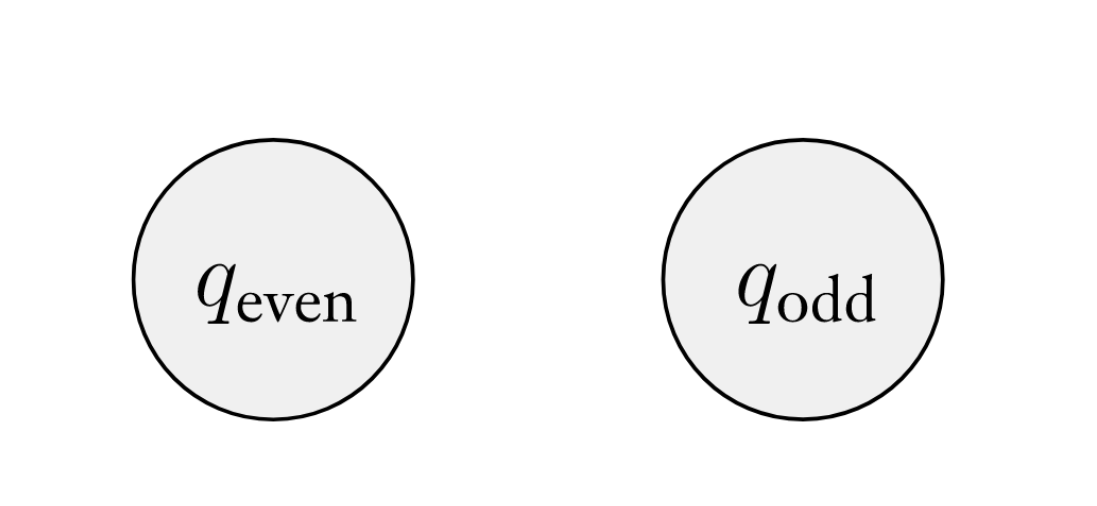
\includegraphics[width=0.8\textwidth]{noTransitions.png}
    \end{center}
\end{frame}

\begin{frame}{Odd number of $\texttt{1}$'s}
    \begin{center}
        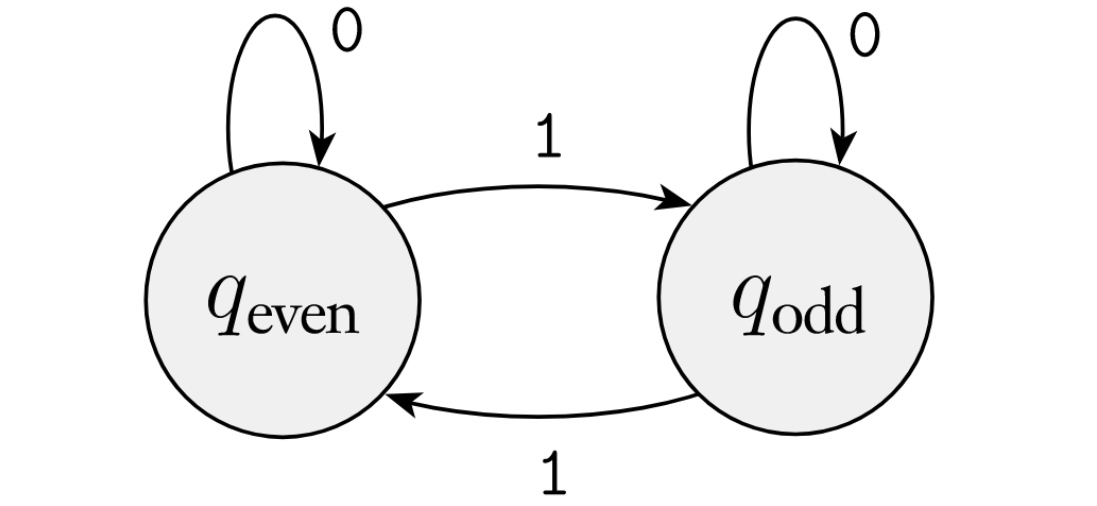
\includegraphics[width=0.8\textwidth]{noAccept.png}
    \end{center}
\end{frame}

% Honestly this aligning isn't bad
\begin{frame}{Odd number of $\texttt{1}$'s}
    \begin{center}
        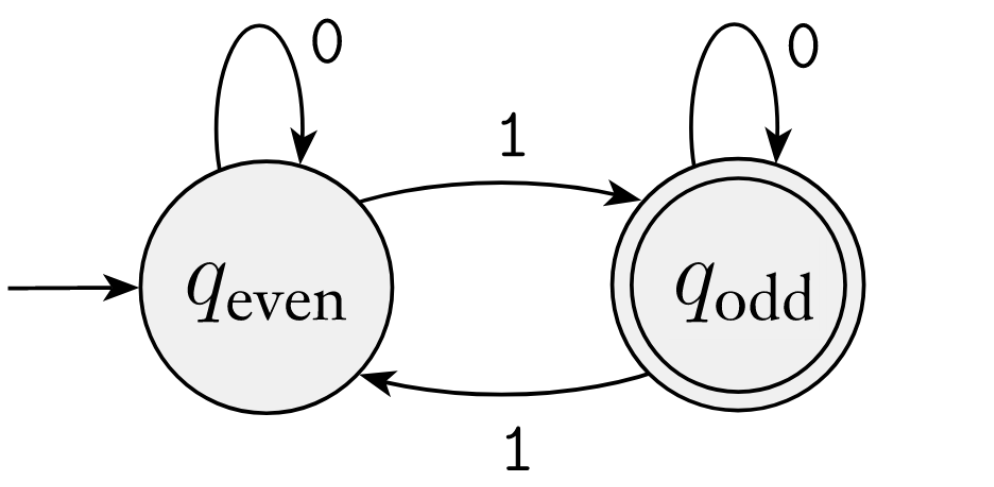
\includegraphics[width=0.8\textwidth]{evenDFA.png}
    \end{center}
\end{frame}

\begin{frame}{}
      \begin{center}
    {\color{sigma@mainblue} \LARGE Questions?}
  \end{center}
\end{frame}

\begin{frame}{Questions!}
    
    \begin{itemize}
        \item Remember those regex from before? \pause
        \item Turns out regex are \textbf{equivalent} to DFAs!! 
        
              Every regex can be turned into a DFA, and vice versa \pause
    \end{itemize}
    
    Try to come up with DFAs for some of the following regular expressions:

    \begin{enumerate}
        \item $\texttt{0}^* + \texttt{0}^* 1 \texttt{0}^*$ 
        \item $( \Sigma \Sigma \Sigma)^*$
        \item $\texttt{0 + 1 + 0} \Sigma^* \texttt{0 + 1} \Sigma^* \texttt{1}$
    \end{enumerate}
\end{frame}

\begin{frame}
  \begin{center}
    {\color{sigma@mainblue} \LARGE See y'all next week!}
  \end{center}
\end{frame}

% % Another frame:
% \begin{frame}
%   % Alternate syntax for frame titles
%   \frametitle{There Is No Largest Prime Number}
%   % Frames can have subtitles:
%   \framesubtitle{The proof uses \textit{reductio ad absurdum}.}
%   % Some frame content:
%   \begin{theorem}
%     There is no largest prime number.
%   \end{theorem}
%   \begin{enumerate}
%     % We do some interesting stuff with the items to make them appear
%     % on sequential slides. See the PDF for how this turns out. The
%     % first item is set to alert on the first slide in red.
%     \item<1-| alert@1> Suppose $p$ were the largest prime number.
%     \item<2-> Let $q$ be the product of the first $p$ primes.
%     \item<3-> Then $q+1$ is not divisible by any of them.
%     \item<4-> But $q + 1$ is greater than $1$, thus divisible by some prime
%     number not in the first $p$ numbers.
%     \item<5-> There exists a prime larger than $p$.
%   \end{enumerate}
% \end{frame}


% \section{RSA}
% \frame{\sectionpage}

% % Similar for subsections:
% \subsection{Some Intuition}
% % And their pages:
% \frame{\subsectionpage}

% \begin{frame}
%   \frametitle{Image}
%   % This is how you'd include an image, centered.
%   \begin{center}
%     
\includegraphics[width=0.25\textwidth]{sigma.png}
%   \end{center}
% \end{frame}

% \subsection{The Math}
% \frame{\subsectionpage}

% \begin{frame}
%   \frametitle{Key Generation}

%   \begin{enumerate}
%     \item Find primes $p$, $q$. Compute $n=pq$.
%     \item Compute $\phi = (p-1)(q-1)$.
%     \item Let $e$ be a number coprime to $n$.
%     \item Compute $d = e^{-1} \pmod{\phi}$.
%     \item $(n,e)$ is the \textbf{public key} tuple, $d$ is the \textbf{private key}.
%   \end{enumerate}

% \end{frame}

% \begin{frame}
%   \frametitle{Message Exchange}

%   \begin{enumerate}
%     % Note that we can use the SIGma colors the template makes
%     % available to us anywhere we'd like:
%     \item To send message $m$ to Alice, Bob computes $c = m^e \pmod{n}$
%       using {\color{sigma@alertred} Alice's public key} $(n,e)$ and sends $c$ to Alice.
%     \item Alice computes $m = c^d \pmod{n}$ to recover $m$.
%   \end{enumerate}
% \end{frame}

% \begin{frame}
%   \frametitle{Some Math Mode Testing}
%   % Some fun with LaTeX Math
%   $$\frac{x^2+3}{y^2+7}$$

%   \[
%     \mathcal L_{\mathcal T}(\vec{\lambda})
%     = \sum_{(\mathbf{x},\mathbf{s})\in \mathcal T}
%       \log P(\mathbf{s}\mid\mathbf{x}) - \sum_{i=1}^m
%       \frac{\lambda_i^2}{2\sigma^2}
%   \]

%   $$\int_0^8 f(x) dx$$
% \end{frame}

% \begin{frame}[fragile]
%   \frametitle{Some Sample Code}

%   \begin{minted}{python}
%     x = 10
%     y = "mystring"
%     print("Hello world!")
%   \end{minted}

% \end{frame}


% \section{Conclusion}
% \frame{\sectionpage}

% \begin{frame}
%   \begin{center}
%     {\color{sigma@mainblue} So long, and thanks for all the fish!}
%   \end{center}
% \end{frame}

\end{document}